%%%%%%%%%%%%%%%%%%%%%%%%%%%%%%%%%%%%%%%%%
% Stylish Article
% LaTeX Template
% Version 2.1 (1/10/15)
%
% This template has been downloaded from:
% http://www.LaTeXTemplates.com
%
% Original author:
% Mathias Legrand (legrand.mathias@gmail.com) 
% With extensive modifications by:
% Vel (vel@latextemplates.com)
%
% License:
% CC BY-NC-SA 3.0 (http://creativecommons.org/licenses/by-nc-sa/3.0/)
%
%%%%%%%%%%%%%%%%%%%%%%%%%%%%%%%%%%%%%%%%%

%----------------------------------------------------------------------------------------
%	PACKAGES AND OTHER DOCUMENT CONFIGURATIONS
%----------------------------------------------------------------------------------------

\documentclass[fleqn,10pt]{SelfArx} % Document font size and equations flushed left

\usepackage[frenchb]{babel} % Specify a different language here - english by default
\usepackage[utf8]{inputenc}
\usepackage{lipsum} % Required to insert dummy text. To be removed otherwise

%----------------------------------------------------------------------------------------
%	COLUMNS
%----------------------------------------------------------------------------------------

\setlength{\columnsep}{0.55cm} % Distance between the two columns of text
\setlength{\fboxrule}{0.75pt} % Width of the border around the abstract

%----------------------------------------------------------------------------------------
%	COLORS
%----------------------------------------------------------------------------------------

\definecolor{color1}{RGB}{0,0,90} % Color of the article title and sections
\definecolor{color2}{RGB}{0,20,20} % Color of the boxes behind the abstract and headings

%----------------------------------------------------------------------------------------
%	HYPERLINKS
%----------------------------------------------------------------------------------------

\usepackage{hyperref} % Required for hyperlinks
\hypersetup{hidelinks,colorlinks,breaklinks=true,urlcolor=color2,citecolor=color1,linkcolor=color1,bookmarksopen=false,pdftitle={Conversion HFR LFR},pdfauthor={Florent GUIOTTE, Paul LE DENN, Brieuc DANIEL, Danchi LI}}

%----------------------------------------------------------------------------------------
%	ARTICLE INFORMATION
%----------------------------------------------------------------------------------------

\JournalInfo{Projets Industriels, B$\textless\textgreater$COM, ESIR, 2016} % Journal information
\Archive{Article technique de restitution} % Additional notes (e.g. copyright, DOI, review/research article)

\PaperTitle{Conversion HFR LFR} % Article title

\Authors{Florent GUIOTTE\textsuperscript{1}, Paul LE DENN\textsuperscript{1}, Brieuc DANIEL\textsuperscript{1}, Danchi LI\textsuperscript{1}\\Olivier LE MEUR\textsuperscript{2}\\Jean-Yves AUBIE\textsuperscript{3}} % Authors

\affiliation{\textsuperscript{1}\textit{Imagerie Numérique, École Supérieure d'Ingénieurs de Rennes, Université de Rennes 1, France\\}
\textsuperscript{2}\textit{École Supérieure d'Ingénieurs de Rennes, Université de Rennes 1, France\\}
\textsuperscript{3}\textit{B$\textless\textgreater$COM, Rennes, France}
} % Author affiliation

\Keywords{Haute fréquence d'image (High Frame Rate, HFR), faible fréquence d'image (Low Frame Rate, LFR), flot optique, conversion} % Keywords - if you don't want any simply remove all the text between the curly brackets
\newcommand{\keywordname}{Mots-Clés} % Defines the keywords heading name

%----------------------------------------------------------------------------------------
%	ABSTRACT
%----------------------------------------------------------------------------------------

\Abstract{Le monde de la vidéo a vu naître de nombreux formats durant ces dernières années. Les technologies ont rapidement évoluée et nous permettent de visionner des vidéos en HD, Full HD et même Ultra HD. 
De la même manière, les cameras permettent de filmer des séquences vidéo HFR avec un rythme d'image de l'ordre de 100 images par seconde — plus fluides que des vidéos LFR — 50 images par secondes. 
Malheureusement, tous les écrans ne sont pas en mesure d'afficher des vidéos enregistrées à de telles fréquences.
Nous travaillons en partenariat avec B$\textless\textgreater$COM pour effectuer la conversion d'une fréquence élevée vers une fréquence adaptée, afin d'obtenir des vidéos compatibles pour tous les écrans.
Une vidéo HFR contient des images plus nettes qu'une vidéo LFR, supprimer une image sur deux provoquerait donc des saccades désagréables à l'œil.
Nous proposons dans notre solution une approche perfectionnée prenant en compte l'effet de flou provoqué par des objets en mouvement.
Cet effet est naturellement présent dans les vidéos LFR et est appelé flou de mouvement ou flou cinétique.
Nous détectons le mouvement dans la vidéo via le calcul d'un flot optique et d'un gradient temporel, puis nous appliquons un traitement pour reproduire le flou cinétique selon le mouvement.\\

The world of video has produced many formats in recent years. Technology has advanced rapidly and allow us to watch videos in HD, Full HD and even Ultra HD.
Similarly, the cameras used to record HFR videos with an image rate of about 100 frames per second — more fluid than LFR video — 50 frames per second.
Unfortunately, all the screens are not able to display these videos recorded at such frequencies.
We partner with B$\textless\textgreater$COM to convert a high frequency to a suitable frequency, in order to get compatible videos for all screens.
A video contains sharper HFR images than LFR video, delete an image on two jerks therefore cause unpleasant to the eye.
We offer our solution in a sophisticated approach taking into account the blur caused by moving objects.
This effect is naturally present in LFR and videos is called motion blur.
We detect motion in the video through calculating an optical flow and a temporal gradient, then apply a treatment to reproduce the motion blur according to the movement.}

%----------------------------------------------------------------------------------------

\begin{document}

\flushbottom % Makes all text pages the same height

\maketitle % Print the title and abstract box

\tableofcontents % Print the contents section

\thispagestyle{empty} % Removes page numbering from the first page

%----------------------------------------------------------------------------------------
%	ARTICLE CONTENTS
%----------------------------------------------------------------------------------------

\section*{Introduction} % The \section*{} command stops section numbering
\addcontentsline{toc}{section}{Introduction} % Adds this section to the table of contents

Les entreprises évoluant dans le domaine du traitement d'image et de la compression vidéo cherchent à développer de nouveaux formats permettant un gain de qualité.
Pour cela, deux paramètres peuvent être améliorés : la qualité spatiale (résolution d'image, compression) et temporelle (haute fréquence d'image).
Ces deux paramètres sont l'objet de travaux au sein de l'institut de recherche technologique B$\textless\textgreater$COM qui a pour objectif de fournir une meilleure sensation d'immersion des spectateurs dans les contenus audiovisuels.
Cet institut de recherche possède un laboratoire étudiant le réalisme des contenus.
Leur but est de développer des outils visant a faciliter la prise en main de ces futurs formats par les professionnels du secteur (cinéma, télévision, jeux, publicité, etc.) et, a terme, par le public.
Parallèlement, les chercheurs de B$\textless\textgreater$COM travaillent sur la possibilité de rendre ces formats lisibles sur des moniteurs non compatibles.
C'est notamment le cas des vidéos enregistrées à une fréquence d'images élevées, typiquement 100 ou 120 images par seconde (ips), non lisibles sur des écrans qui ne peuvent afficher que 50 ou 60 ips maximum.
Dans cette optique, nous sommes amenés à proposer une solution permettant de réduire de moitié la fréquence d'image de vidéos HFR sans détériorer la fluidité des mouvements pour le spectateur.
En HFR, l'intervalle de temps entre 2 images consécutives est très court, les déplacements des objets entre les 2 images le sont donc également.
La succession des images donne alors une impression de mouvement très proche de la réalité.
En LFR, cet intervalle de temps étant plus important, la fluidité est obtenue par un rendu plus flou des objets en mouvements (figure 1). Il s'agit du flou cinétique, provoqué par le temps de pose plus long de la camera lors de la capture d'une image.
Pour réduire la fréquence d'image, la solution intuitive consisterait a supprimer une image sur deux. Néanmoins, des travaux réalises auparavant à B$\textless\textgreater$COM ont montré que cette solution n'est pas satisfaisante car elle ne permet pas de retrouver le flou cinétique.
La vidéo semble alors très hachée.
De même, des traitements globaux comme une combinaison linéaire classique d'images successives n'élimine pas suffisamment les saccades.
Dans ce document, nous étudions la manière dont il est possible de simuler le flou cinétique localement sur les images.
Les deux solutions que nous proposons se basent sur l'estimation du mouvement dans la vidéo originale.
La première consiste à reprendre l'idée d'une combinaison de plusieurs images, cette fois avec une accélération matérielle.
La seconde méthode est l'application de flous cinétiques sur les objets qui se déplacent grâce à des gradient temporels.

%------------------------------------------------

\section{Méthodes}

\begin{figure*}[ht]\centering % Using \begin{figure*} makes the figure take up the entire width of the page
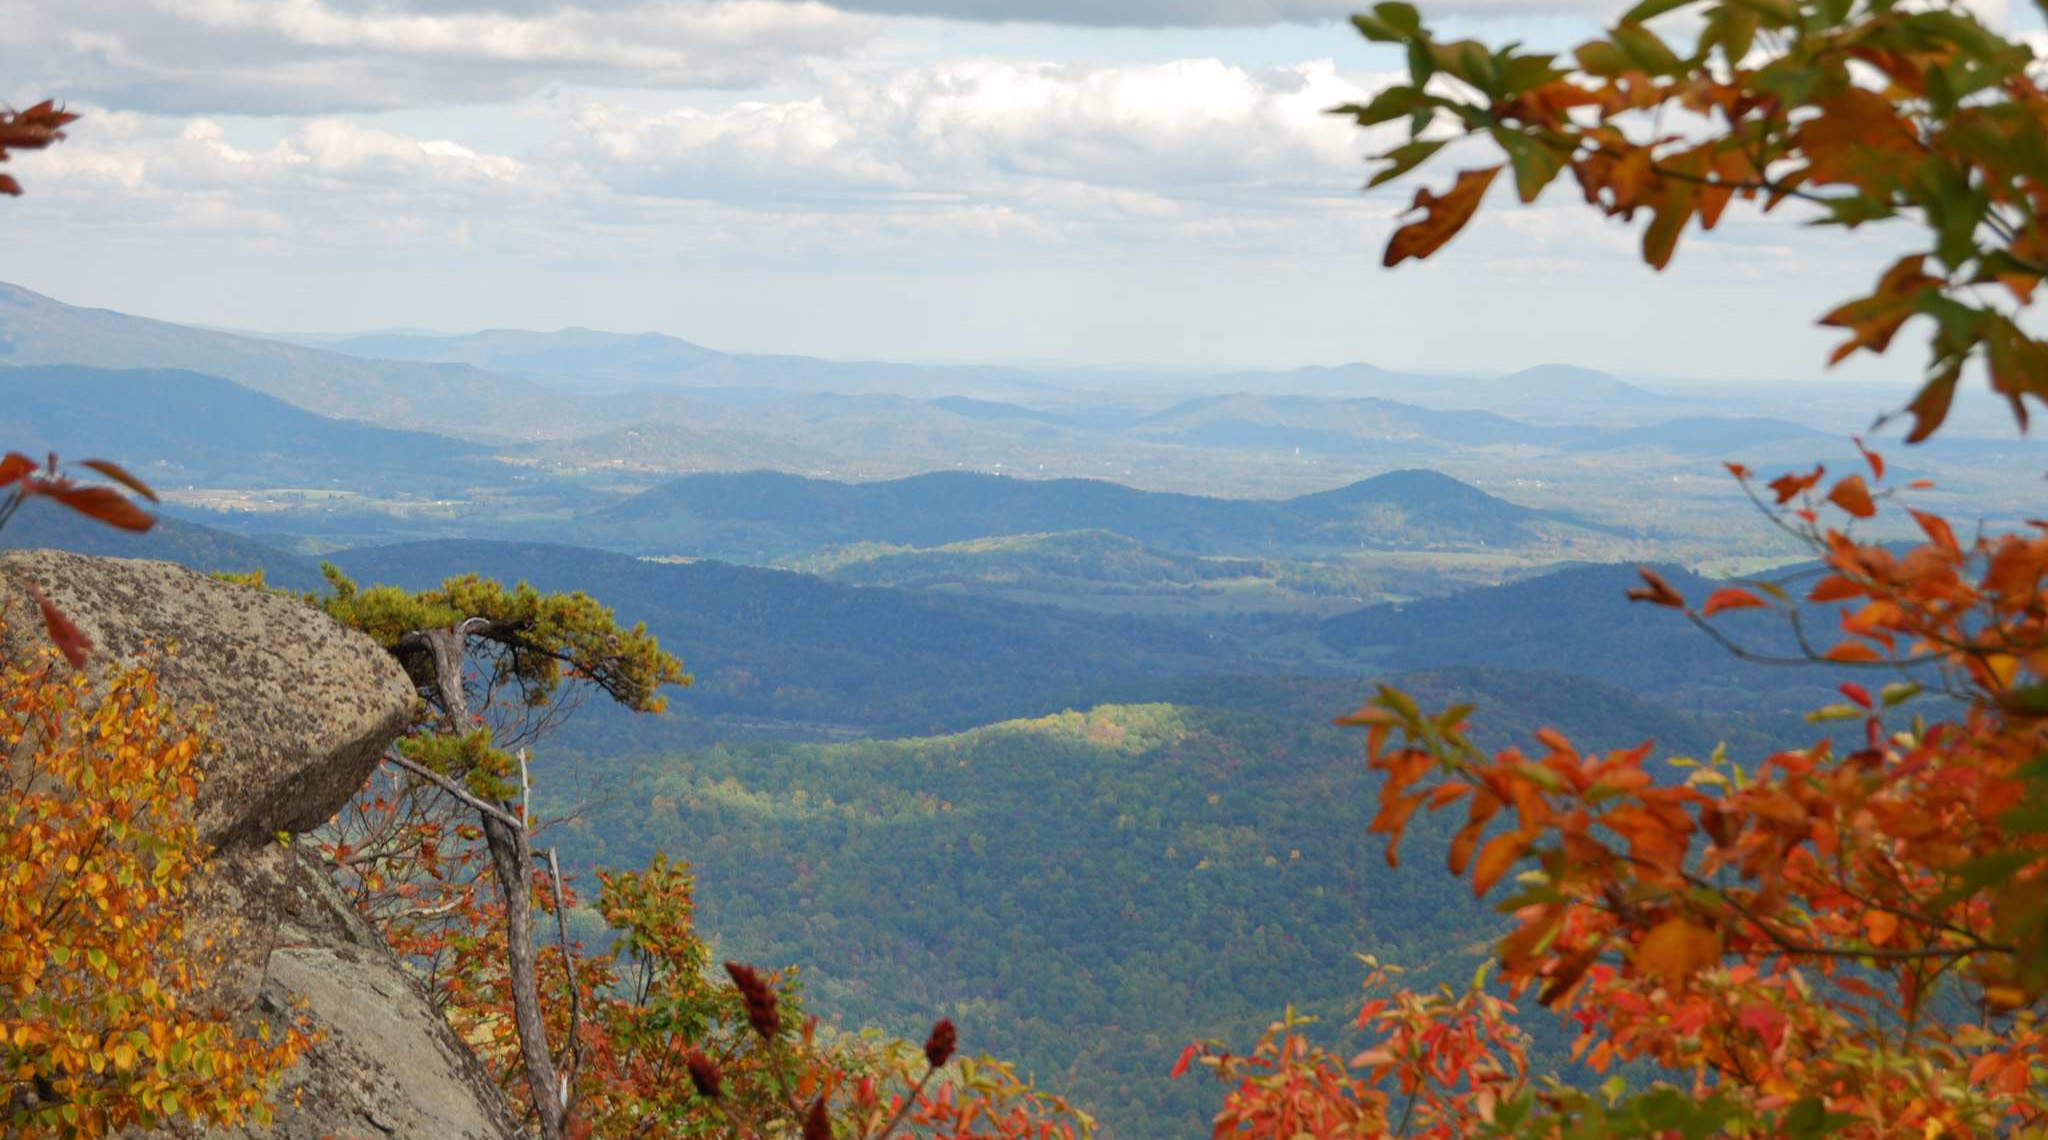
\includegraphics[width=\linewidth]{view}
\caption{Wide Picture}
\label{fig:view}
\end{figure*}

\lipsum[4] % Dummy text

\begin{equation}
\cos^3 \theta =\frac{1}{4}\cos\theta+\frac{3}{4}\cos 3\theta
\label{eq:refname2}
\end{equation}

\lipsum[5] % Dummy text

\begin{enumerate}[noitemsep] % [noitemsep] removes whitespace between the items for a compact look
\item First item in a list
\item Second item in a list
\item Third item in a list
\end{enumerate}

\subsection{Les méthodes utilisées}

\lipsum[6] % Dummy text

\paragraph{Paragraph} \lipsum[7] % Dummy text
\paragraph{Paragraph} \lipsum[8] % Dummy text

\subsection{Choix des méthodes utilisées}

\lipsum[9] % Dummy text

\begin{figure}[ht]\centering
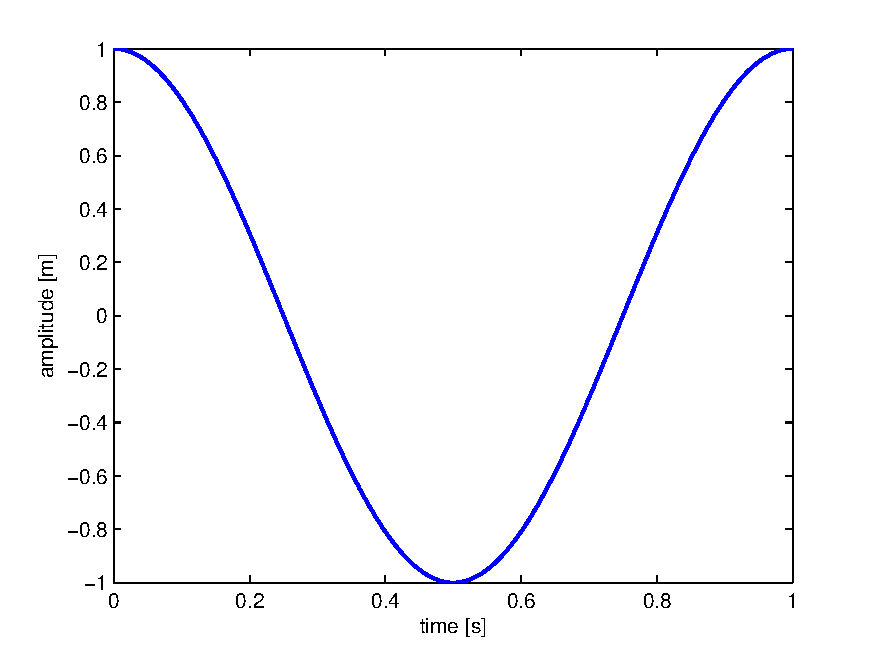
\includegraphics[width=\linewidth]{results}
\caption{In-text Picture}
\label{fig:results}
\end{figure}

Reference to Figure \ref{fig:results}.
\subsection{Avantage et contraintes des méthodes}
\subsection{Pourquoi les méthodes choisies permettent de répondre à la problématique}

%------------------------------------------------

\section{Résultats et Discussion}

\lipsum[10] % Dummy text

\subsection{Phase d'annonce}

\lipsum[11] % Dummy text

\begin{table}[hbt]
\caption{Table of Grades}
\centering
\begin{tabular}{llr}
\toprule
\multicolumn{2}{c}{Name} \\
\cmidrule(r){1-2}
First name & Last Name & Grade \\
\midrule
John & Doe & $7.5$ \\
Richard & Miles & $2$ \\
\bottomrule
\end{tabular}
\label{tab:label}
\end{table}

\subsection{Les clés de lecture}

\lipsum[12] % Dummy text

\begin{description}
\item[Word] Definition
\item[Concept] Explanation
\item[Idea] Text
\end{description}

\subsubsection{Pas d'analyse}

\lipsum[13] % Dummy text

\begin{itemize}[noitemsep] % [noitemsep] removes whitespace between the items for a compact look
\item First item in a list
\item Second item in a list
\item Third item in a list
\end{itemize}

\subsection{Subsection}

\lipsum[15-23] % Dummy text

%------------------------------------------------

\section{Conclusion}
\subsection{Rappel de la question/problématique}
\subsection{Présentation/interprétation des résultats et limite}
\subsection{ouverture}

%------------------------------------------------
\phantomsection
\section*{Acknowledgments} % The \section*{} command stops section numbering

\addcontentsline{toc}{section}{Acknowledgments} % Adds this section to the table of contents

So long and thanks for all the fish \cite{Figueredo:2009dg}.

%----------------------------------------------------------------------------------------
%	REFERENCE LIST
%----------------------------------------------------------------------------------------
\phantomsection
\bibliographystyle{unsrt}
\bibliography{sample}

%----------------------------------------------------------------------------------------

\end{document}